\section{Experimental Results}
\label{sec:experimentalResults}

\subsection{Curriculum learning with aerial imagery}
\label{sec:results_curriculum_learning_aerial_imagery}

In Experiment E1, the road detection system have been trained on four different patch datasets. The system's performance for each of these datasets are displayed in Figure \ref{fig:E1_curriculum_norway}. A comparison of the test loss per epoch is displayed in Figure \ref{fig:E1_curr_norway_loss}, whereas the final performance of each network is shown by a precision and recall curve in Figure \ref{fig:E1_curr_norway_pr}. The network configuration used for the tests was identical, as well as the number of training examples seen while training. The performance gap between the results, comes from the first stage of the patch datasets, where different difficulty threshold $D_0$ have been used.\\

\begin{figure}
\begin{subfigure}{0.48\textwidth}
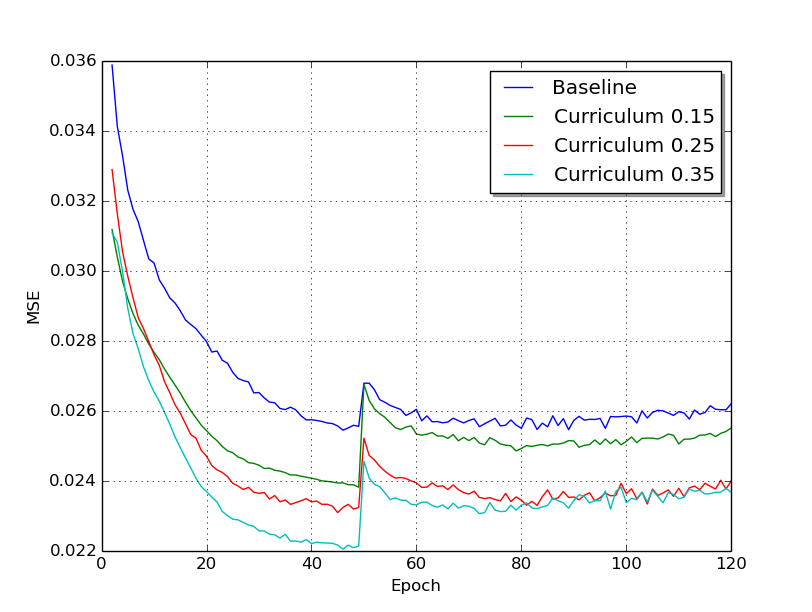
\includegraphics[width=\linewidth]{figs/E1/E1-lc.png}
\caption{Comparison of test loss} \label{fig:E1_curr_norway_loss}
\end{subfigure}
\hspace*{\fill} % separation between the subfigures
\begin{subfigure}{0.48\textwidth}
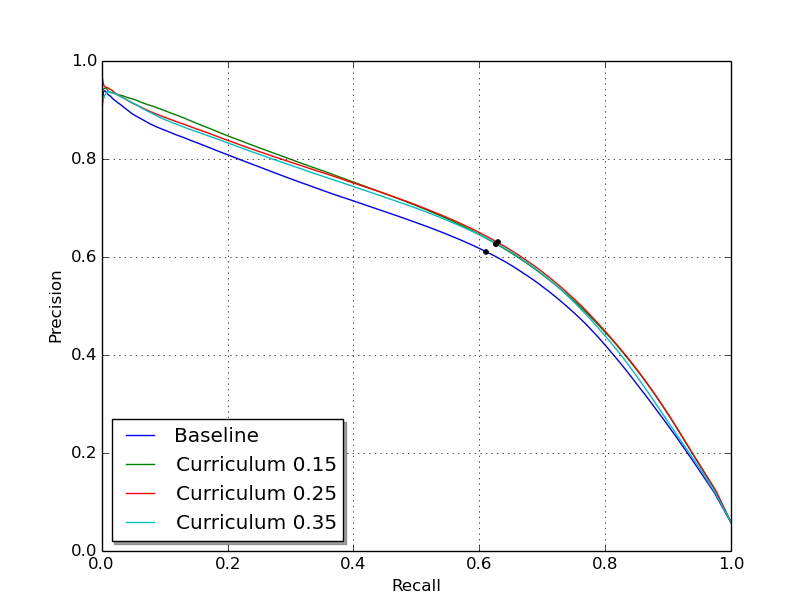
\includegraphics[width=\linewidth]{figs/E1/E1-pr.png}
\caption{Precision and recall comparisons.} \label{fig:E1_curr_norway_pr}
\end{subfigure}
\hspace*{\fill} % separation between the subfigures
\caption{E1 - Performance of curriculum learning at different thresholds, $D_{0}$ for Norwegian Roads Dataset Vbase} \label{fig:E1_curriculum_norway}
\end{figure}

Observing the plots in Figure \ref{fig:E1_curr_norway_loss}, the switch between stage 0 and stage 1, is clearly visible at epoch 50. The increase in test loss is most severe in the datasets formed by a curriculum strategy. Leading up epoch 50, the curriculum plots show an increasing gap in test performance against the baseline plot. After the switch the curriculum datasets still outperform the baseline dataset, even though the training set distribution of stage 1 are the same for all patch datasets.\\

Furthermore, the networks trained with a curriculum strategy shows an improved precision for all levels of recall compared to the baseline. \todo{Not so different here}\\

An interesting trend between the thresholds $D_0$ and the loss, is that decreasing the difficulty threshold, does not necessarily produce better results. The patch dataset \textit{Curriculum 0.15} has the easiest first stage, yet performs worse than \textit{Curriculum 0.25} and \textit{Curriculum 0.35} \todo{Generalize, easier examples reduce variability of training set, generalize worse. Discussion?}. \\

\todo[inline]{Need to place distribution charts somewhere}


A similar experiment was also performed on the Massachusetts Roads Dataset. In Experiment E2, networks are trained with three different patch datasets. The first stage of the baseline dataset have a first stage constructed by random sampling, which means that no examples were filtered out because of estimated difficulty. The curriculum dataset has a difficulty threshold $D_0$ of 0.25, which exclude every example with a estimated difficulty above 0.25 from the first stage. In contrast, the anti-curriculum patch dataset only have examples with a difficulty above 0.25 \todo{Mention, the non-road patches, and why non-road examples have been included}.\\


The results from this experiment can be seen in \ref{fig:E2_curriculum_mass}. Also for this dataset,  \\
\begin{figure}
\begin{subfigure}{0.48\textwidth}
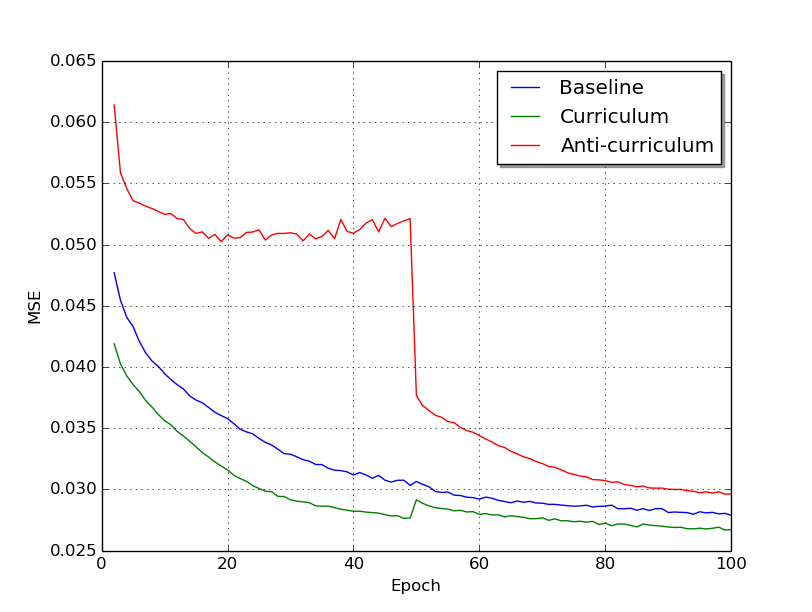
\includegraphics[width=\linewidth]{figs/E2/E2-lc.png}
\caption{Comparison of test loss} \label{fig:E2_curr_mass_loss}
\end{subfigure}
\hspace*{\fill} % separation between the subfigures
\begin{subfigure}{0.48\textwidth}
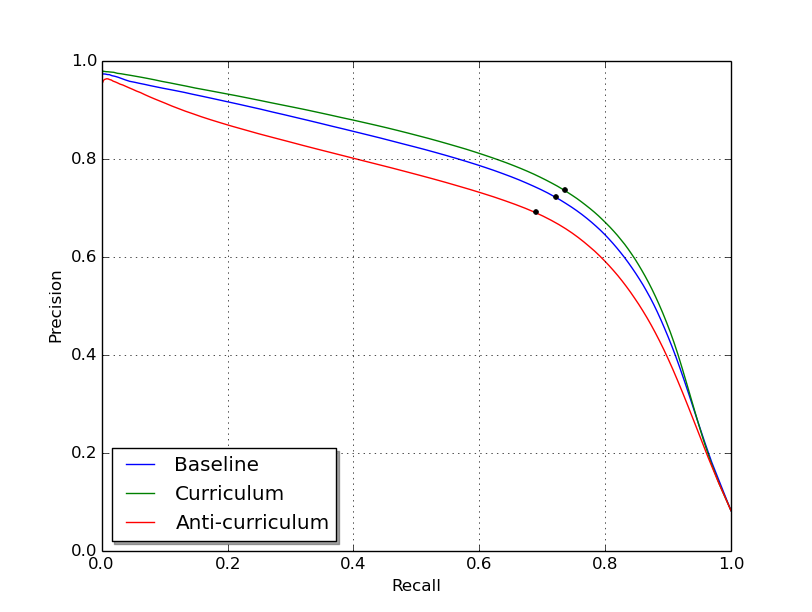
\includegraphics[width=\linewidth]{figs/E2/E2-pr.png}
\caption{Precision and recall comparisons.} \label{fig:E2_curr_mass_pr}
\end{subfigure}
\hspace*{\fill} % separation between the subfigures
\caption{E2 - Performance of curriculum learning and anti-curriculum learning for Massachusetts Roads Dataset} \label{fig:E2_curriculum_mass}
\end{figure}

\begin{table}[htp]
\caption{Curriculum learning results.}
\begin{center}
\begin{adjustbox}{max width=\textwidth}
\begin{tabular}{+l ^l ^l ^r}\hline
\rowstyle{\bfseries}
  Experiment & $\mathbf{D_0}$ & Dataset & Breakeven\\\hline
  Baseline & 1.0 & Norwegian & 0.6105 \\
  Curriculum &0.15 & Norwegian & 0.6264 \\
  Curriculum &0.25 & Norwegian & \textbf{0.6292} \\
  Curriculum &0.35 & Norwegian & 0.6269 \\\hline
  Baseline &1.0& Massachusetts & 0.7211 \\
  Curriculum &0.25& Massachusetts & 0.\textbf{7353} \\
  Anti-curriculum &0.25 & Massachusetts & 0.6904 \\\hline
\end{tabular}
\end{adjustbox}
\end{center}
\label{tab:results_curriculum_learning_breakeven}
\end{table}

\subsection{Bootstrapping for imagery with noisy labels}
\label{sec:results_bootstrapping}
\begin{figure}[!ht]
\begin{subfigure}{0.48\textwidth}
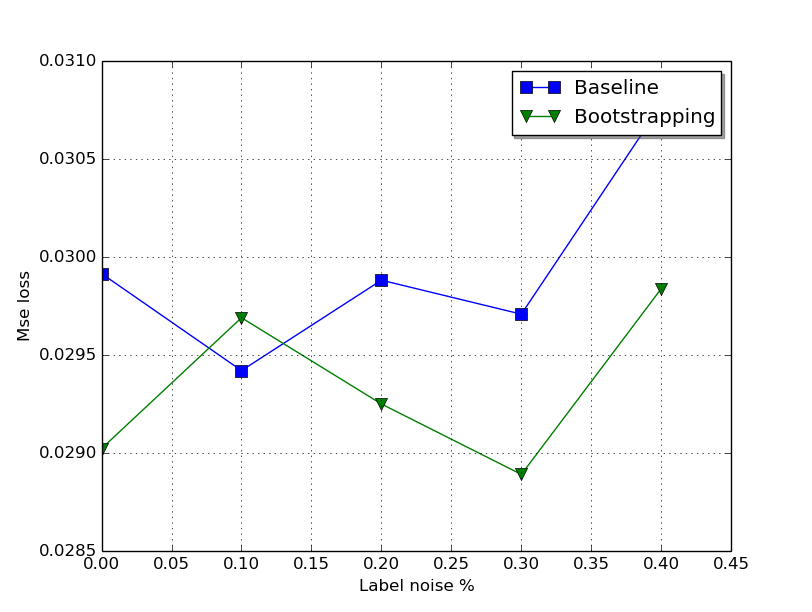
\includegraphics[width=\linewidth]{figs/E3/E3_lc_noise.png}
\caption{MSE test loss} \label{fig:E3_boot_mass_loss}
\end{subfigure}
\hspace*{\fill} % separation between the subfigures
\begin{subfigure}{0.48\textwidth}
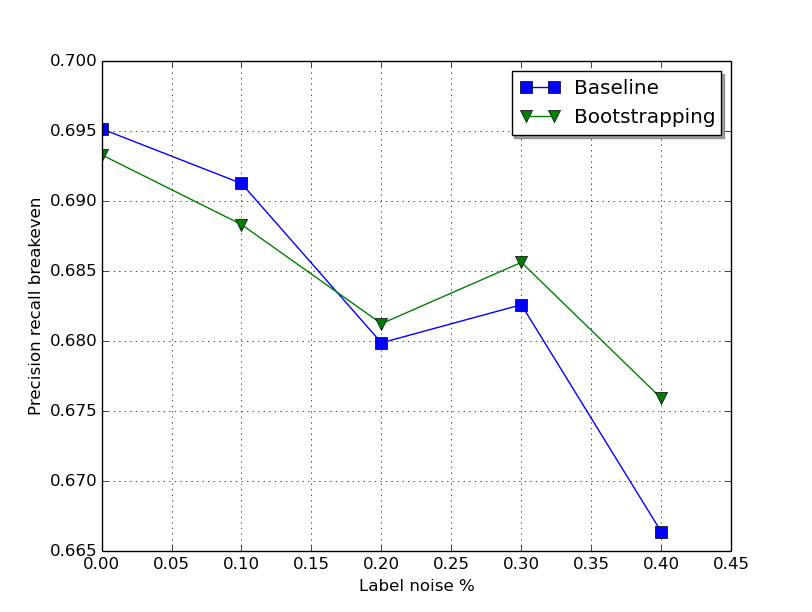
\includegraphics[width=\linewidth]{figs/E3/E3_pr_noise.png}
\caption{Precision and recall breakeven} \label{fig:E3_boot_mass_pr}
\end{subfigure}
\hspace*{\fill} % separation between the subfigures
\caption{E4 - Robustness of bootstrapping for increasing amount of label noise. Massachusetts Roads Dataset} \label{fig:E3_boot_mass}
\end{figure}

\begin{figure}[!ht]
\begin{subfigure}{0.48\textwidth}
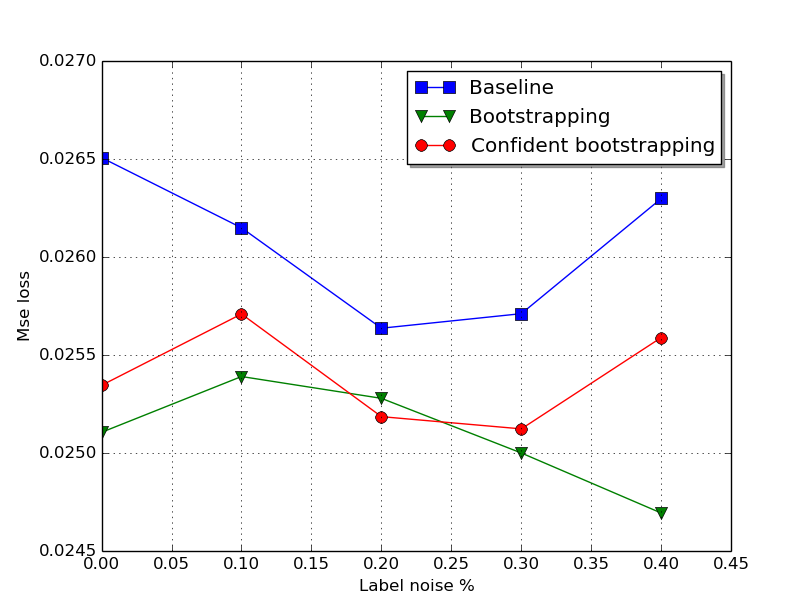
\includegraphics[width=\linewidth]{figs/E5/E5_lc_noise.png}
\caption{MSE test loss} \label{fig:E5_boot_norway_loss}
\end{subfigure}
\hspace*{\fill} % separation between the subfigures
\begin{subfigure}{0.48\textwidth}
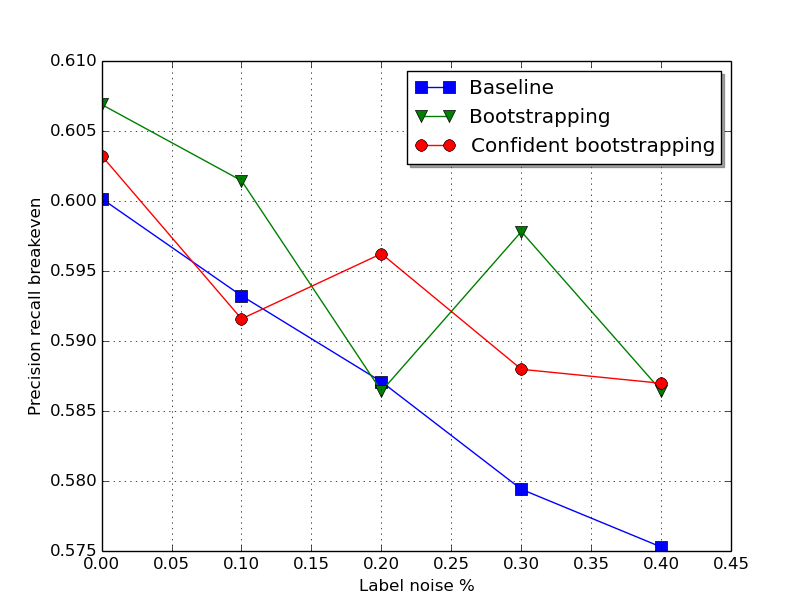
\includegraphics[width=\linewidth]{figs/E5/E5_pr_noise.png}
\caption{Precision and recall breakeven} \label{fig:E5_boot_norway_pr}
\end{subfigure}
\hspace*{\fill} % separation between the subfigures
\caption{E4 - Robustness of bootstrapping for increasing amount of label noise. Norway Roads Dataset} \label{fig:E5_boot_norway}
\end{figure}

\begin{figure}[!ht]
\begin{subfigure}{0.48\textwidth}
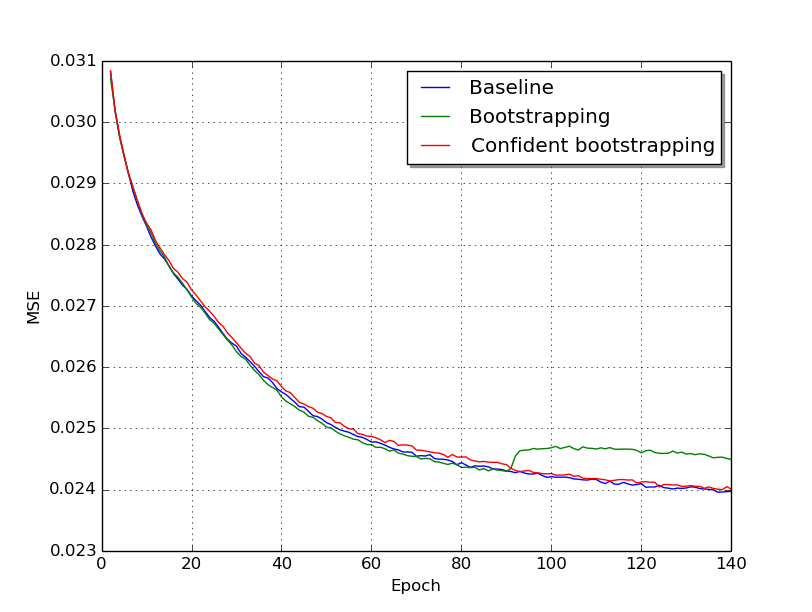
\includegraphics[width=\linewidth]{figs/E4/E4_lc.png}
\caption{MSE test loss} \label{fig:E4_boot_norway_vbase_loss}
\end{subfigure}
\hspace*{\fill} % separation between the subfigures
\begin{subfigure}{0.48\textwidth}
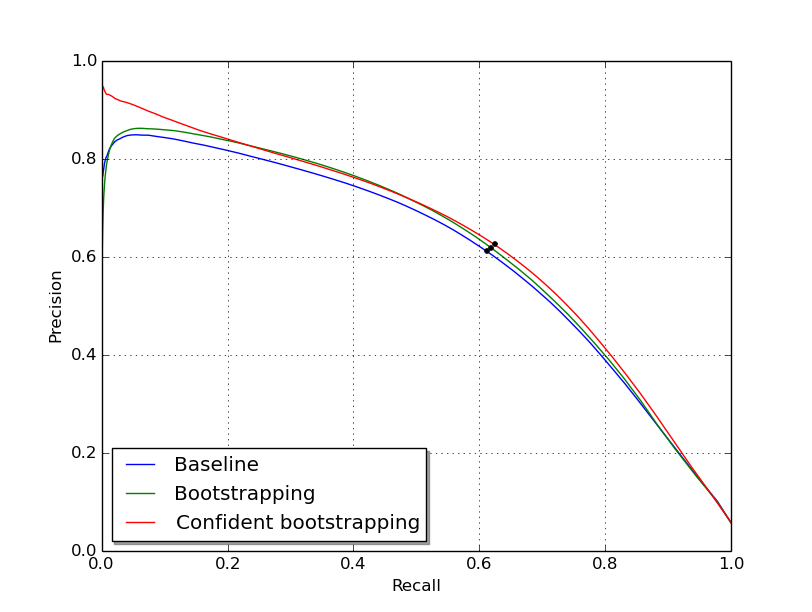
\includegraphics[width=\linewidth]{figs/E4/E4_pr.png}
\caption{Precision and recall comparison.} \label{fig:E4_boot_norway_vbase_pr}
\end{subfigure}
\hspace*{\fill} % separation between the subfigures
\caption{E4 - Comparison of loss functions for Norway Roads Dataset Vbase. The training set consists of labels with both registration and omission noise.} \label{fig:E4_boot_norway_vbase}
\end{figure}

\subsection{Road detection system}
\label{sec:results_road_detection_system}
Nonetheless, the images in Figure \ref{fig:result} illustrates the current performance of the system. In this particular test image, the model is able to identify the majority of the roads present, except for a small gravel road on the right side of the image. There are also a lot of prediction errors, such as roads being disconnected, and prediction artefacts in the forest areas. An interesting observation is that the model also correctly predicts small private roads leading up to houses present in the image. Furthermore, the model detects construction roads in the upper left corner. Since these roads are not present in the label image, the model is penalized for these predictions by the cross-entropy loss function.\\

\begin{figure}[!ht]
\begin{subfigure}{0.48\textwidth}
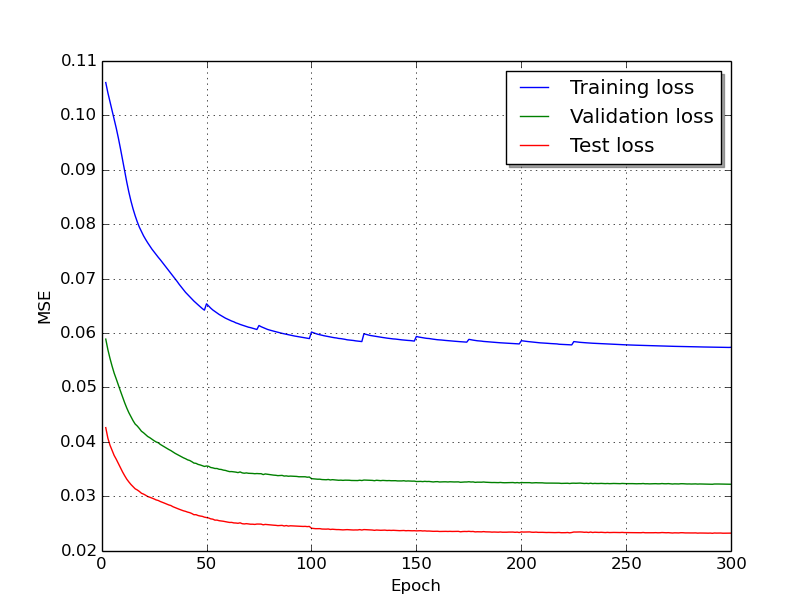
\includegraphics[width=\linewidth]{figs/E6/E6_lc_loss.png}
\caption{MSE loss} \label{fig:E6_performance_mass_lc}
\end{subfigure}
\hspace*{\fill} % separation between the subfigures
\begin{subfigure}{0.48\textwidth}
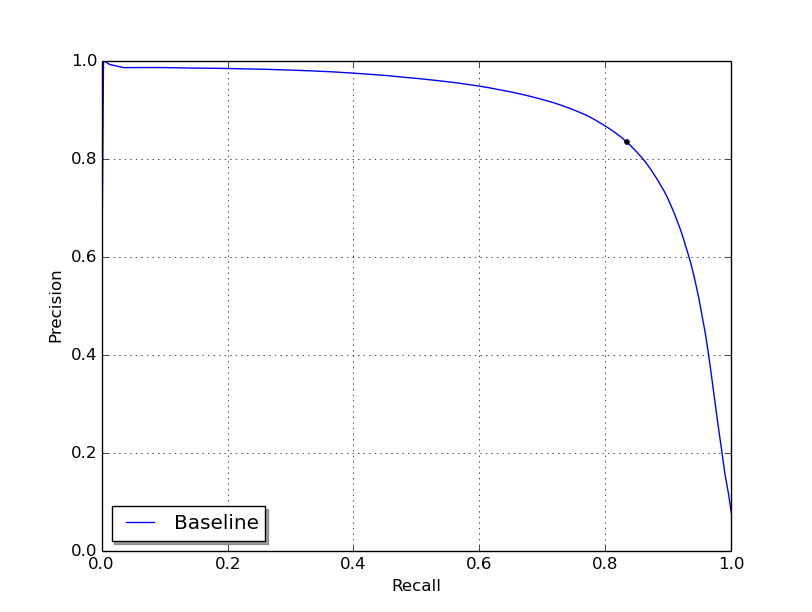
\includegraphics[width=\linewidth]{figs/E6/E6_pr.png}
\caption{Precision and recall and breakeven.} \label{fig:E6_performance_mass_pr}
\end{subfigure}
\hspace*{\fill} % separation between the subfigures
\caption{E6 - Performance of road detection system trained with Massachusetts Roads Dataset} \label{fig:E6_performance_mass}
\end{figure}

\begin{figure}
\begin{subfigure}{0.48\textwidth}
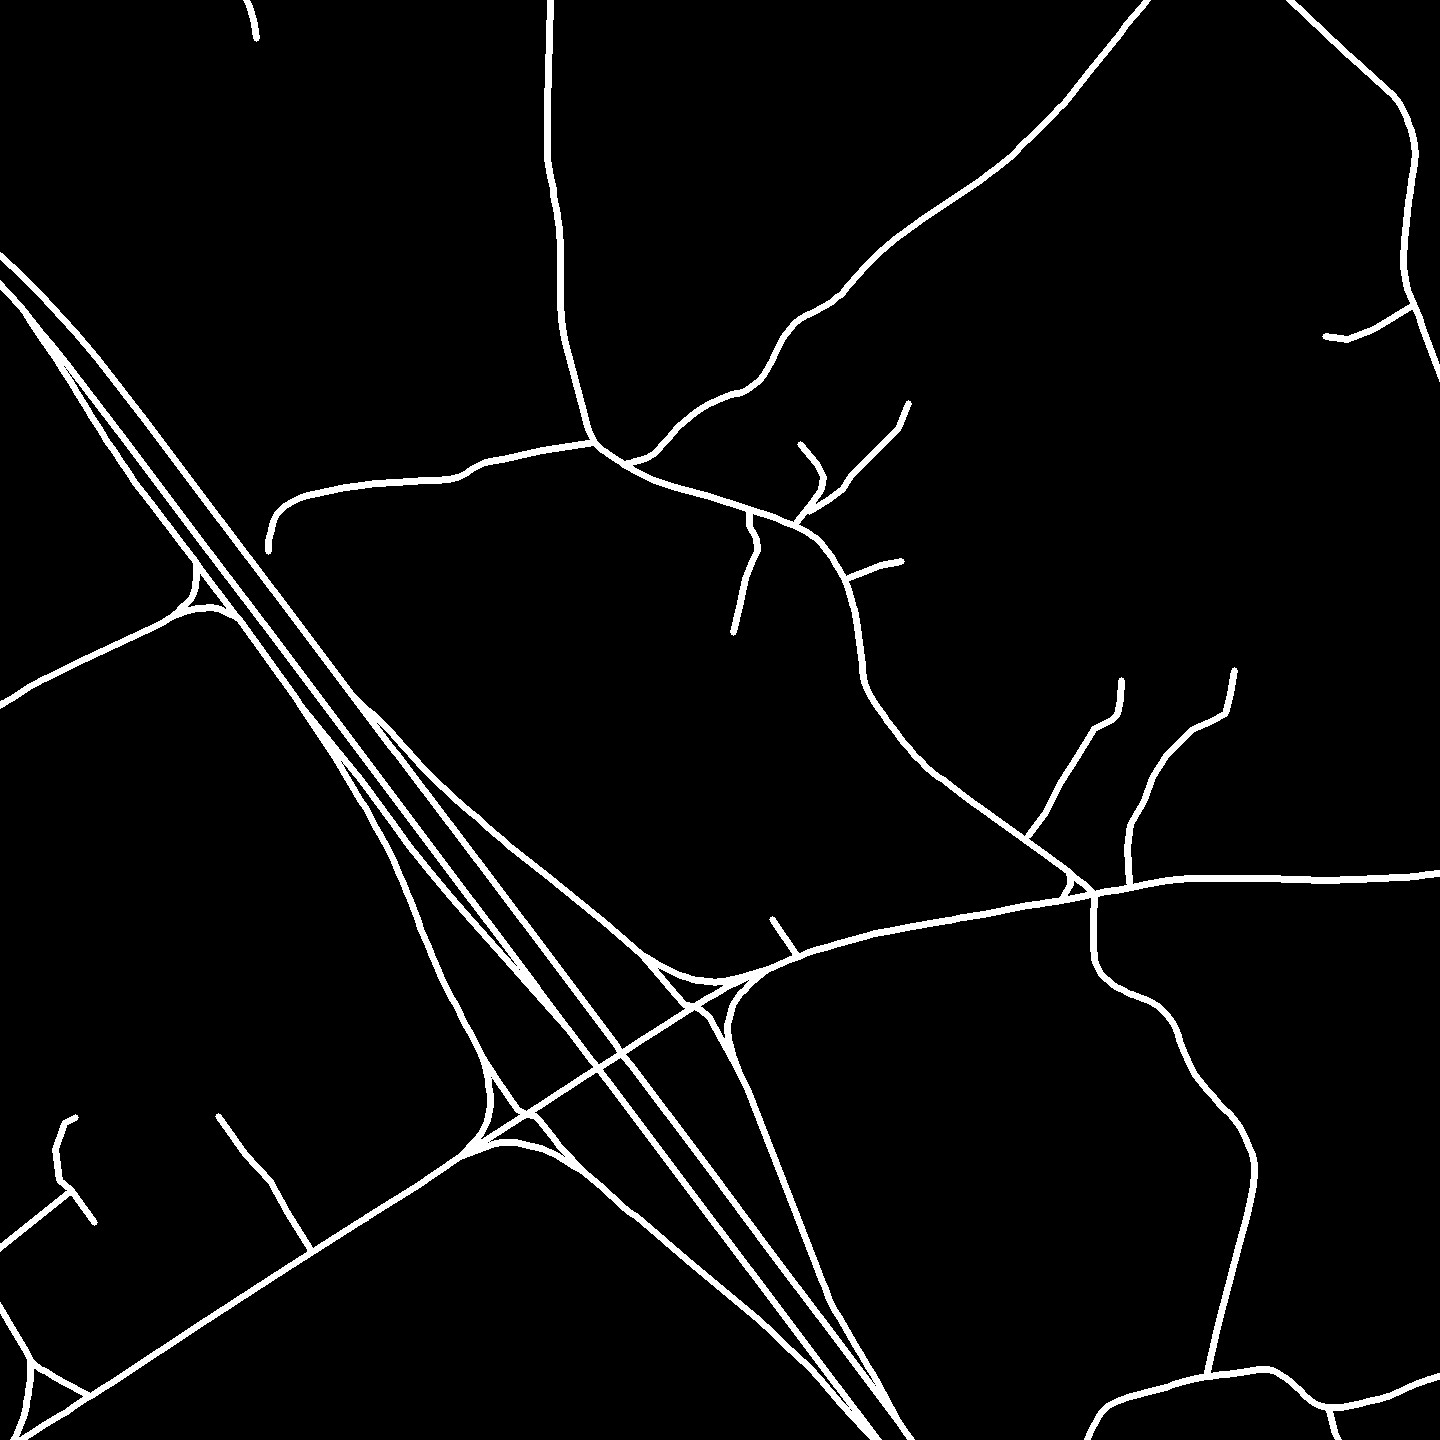
\includegraphics[width=\textwidth]{figs/E6/E6-label.jpg}
\caption{Label image.} \label{fig:E6_label_iamge}
\vspace{0.5cm} % separation vertically between the subfigures
\end{subfigure}
\hspace*{\fill} % separation between the subfigures
\begin{subfigure}{0.48\textwidth}
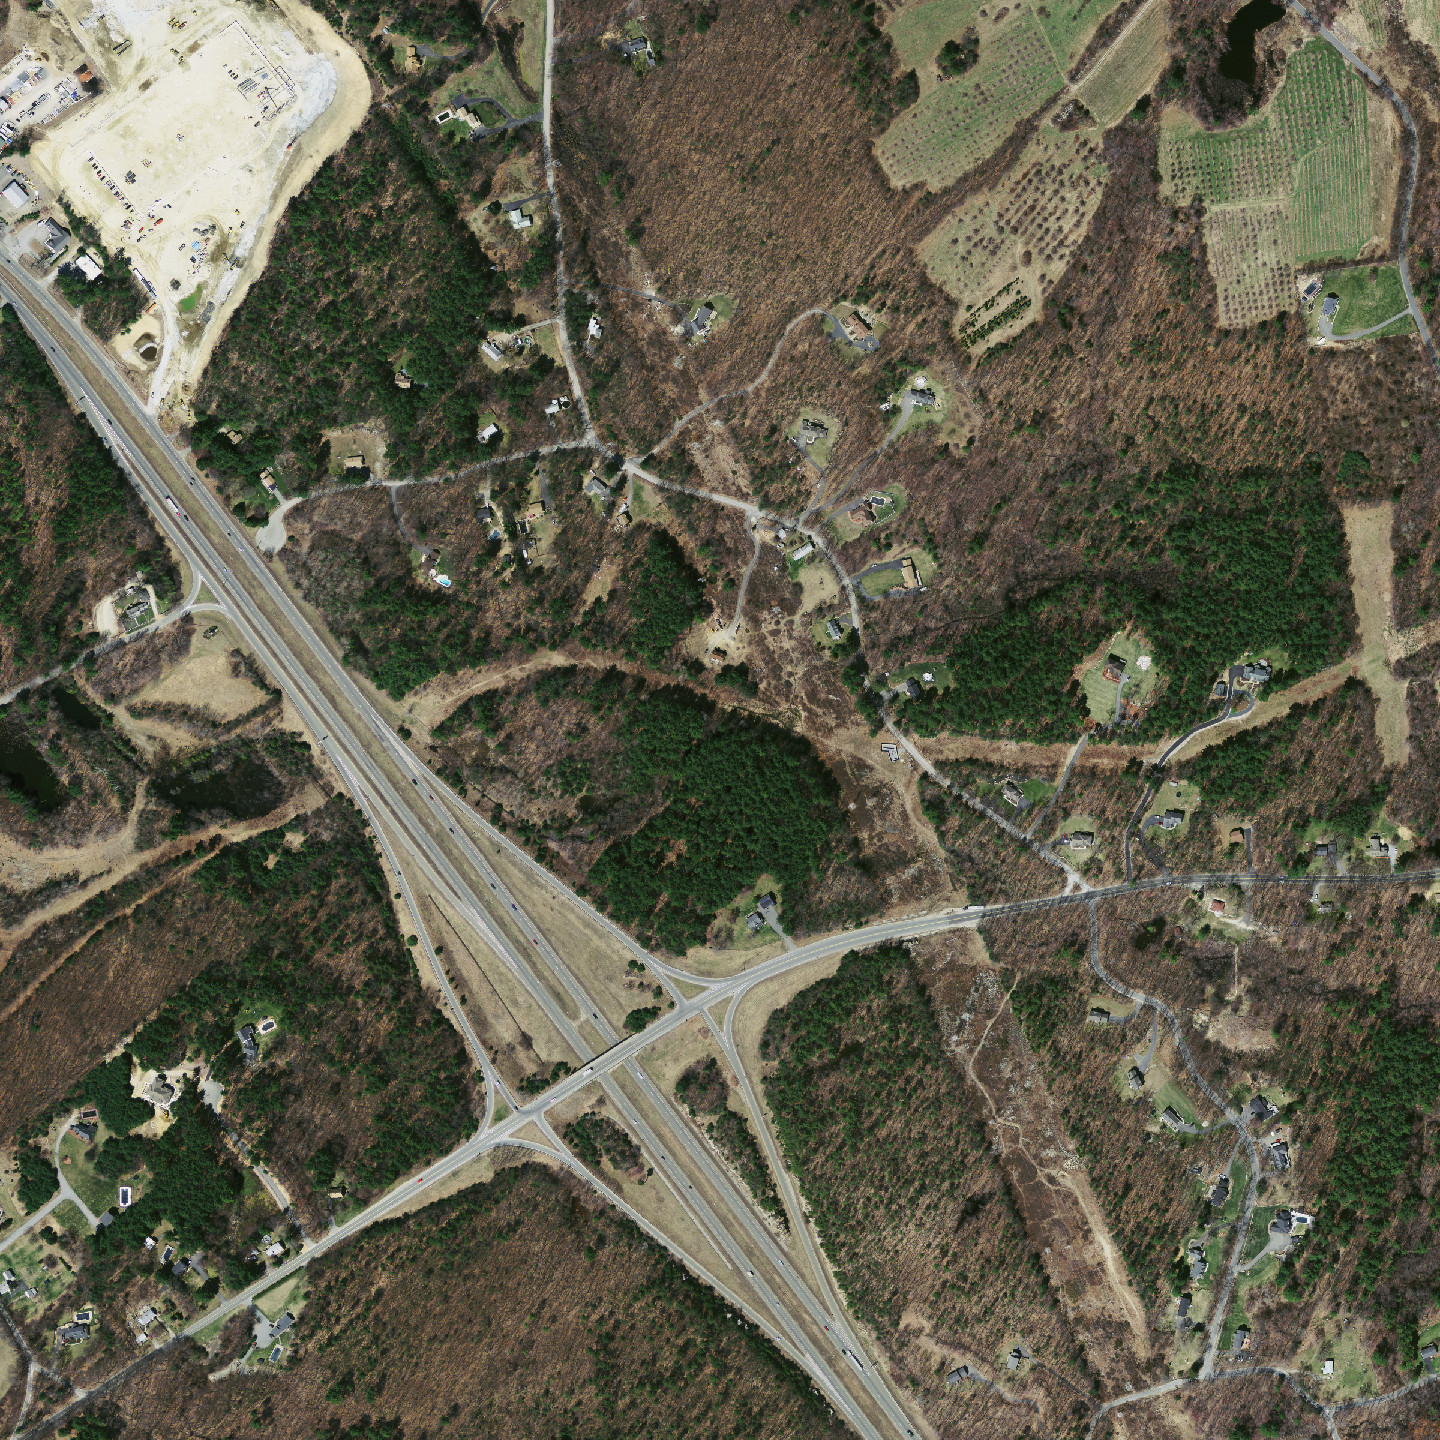
\includegraphics[width=\textwidth]{figs/E6/E6-image.jpg}
\caption{Aerial image.} \label{fig:E6_aerial_image}
\vspace{0.5cm} % separation vertically between the subfigures
\end{subfigure}

\begin{subfigure}{0.48\textwidth}
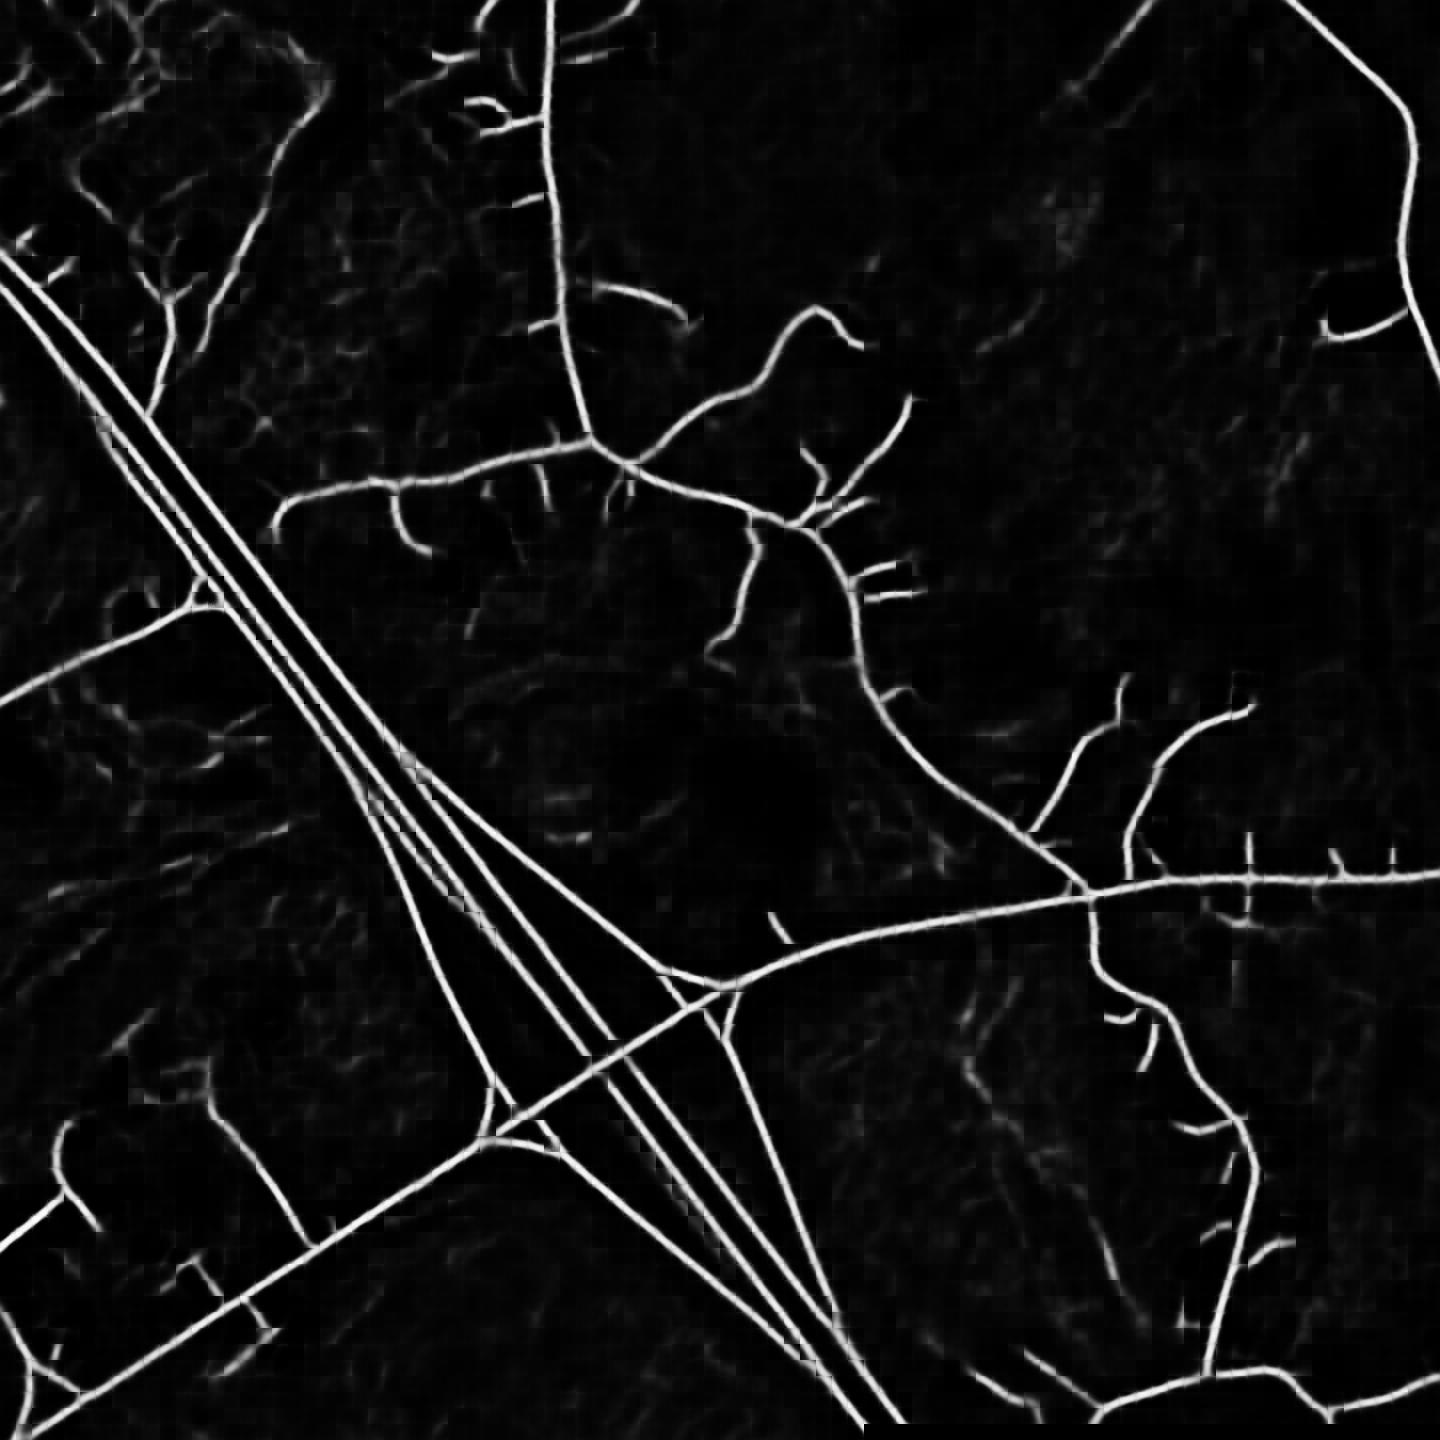
\includegraphics[width=\textwidth]{figs/E6/E6-pred.jpg}
\caption{Model predictions.} \label{fig:E6_model_predictions}
\end{subfigure}
\hspace*{\fill} % separation between the subfigures
\begin{subfigure}{0.48\textwidth}
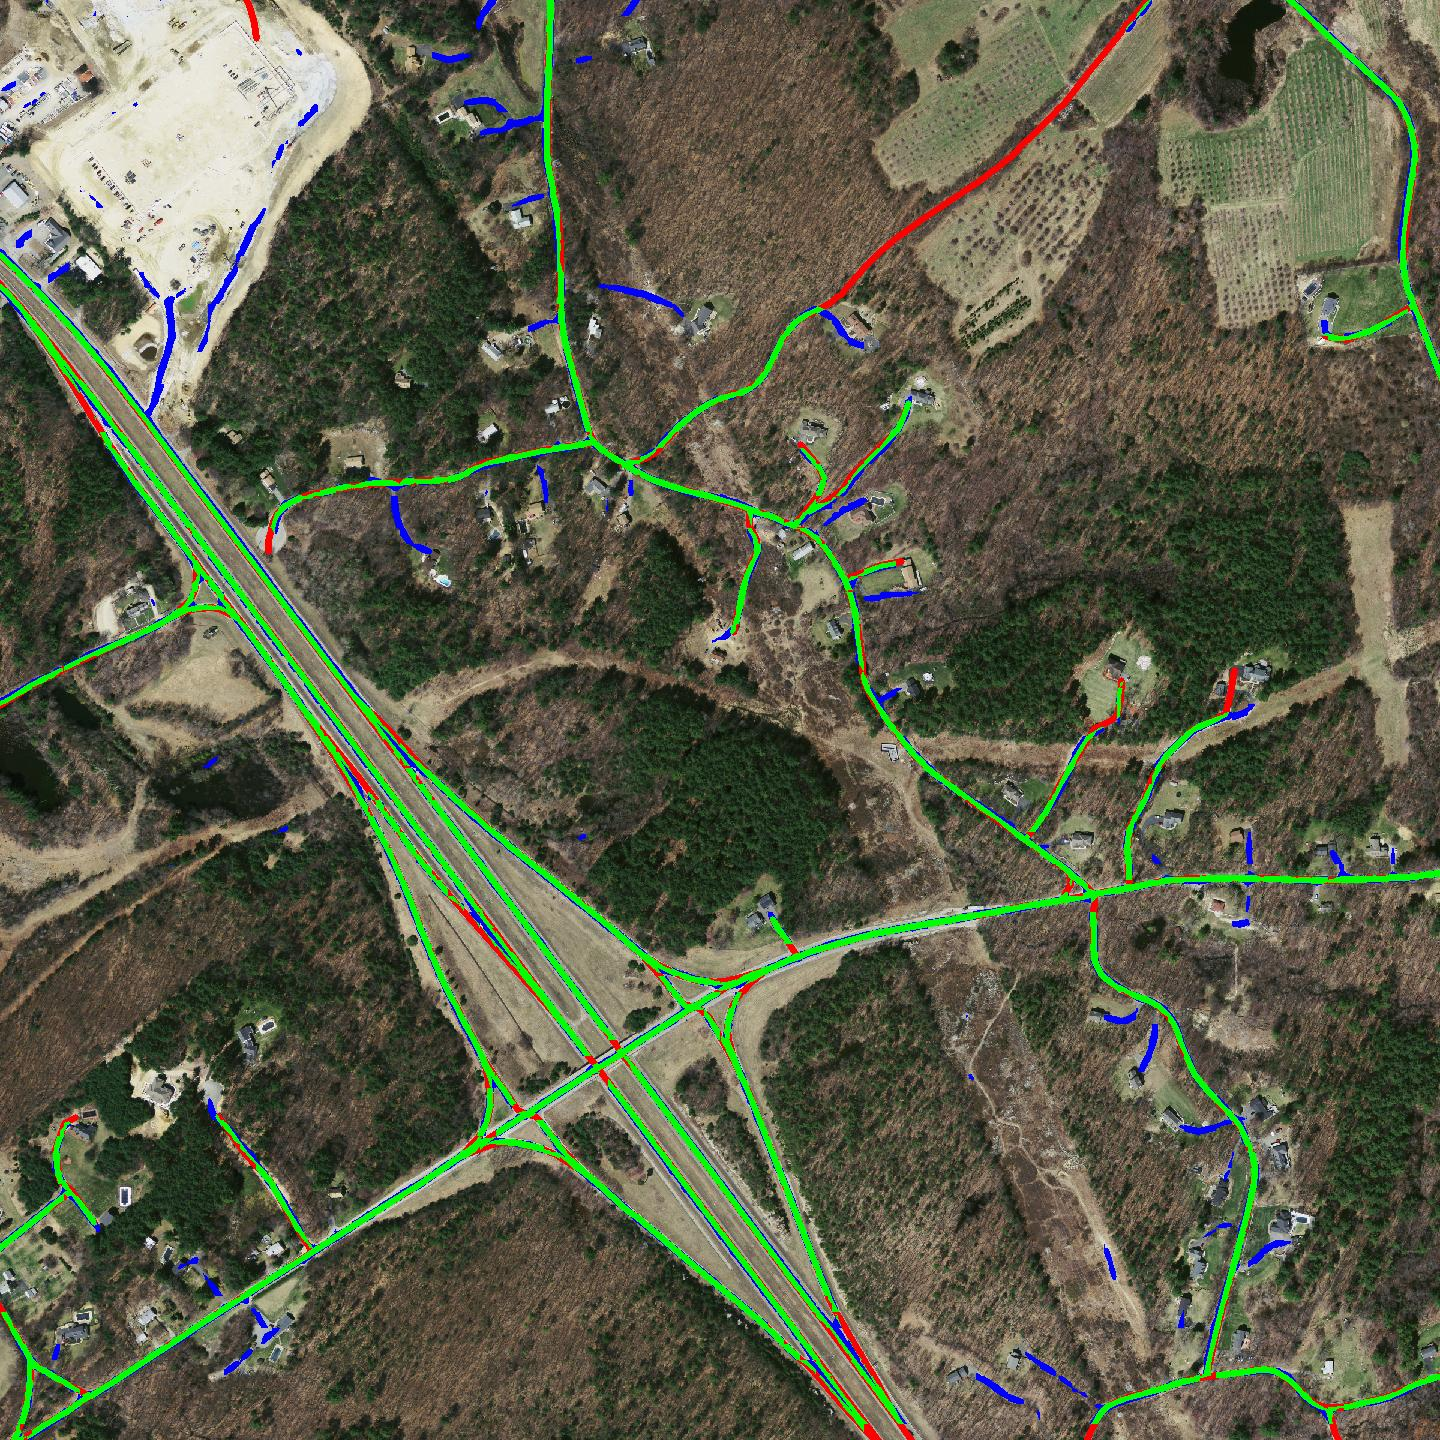
\includegraphics[width=\textwidth]{figs/E6/E6-hit.jpg}
\caption{Prediction hit and miss image.} \label{fig:E6_hit_iamge}
\end{subfigure}
\caption{E6 - Example of model's road detection performance. The aerial image is part of the test set in Massachusetts Roads Dataset} \label{fig:E6_performance}
\end{figure}




\todo[inline]{Choose what to present}
\todo[inline]{Present results for each experiment}
\todo[inline]{Avoid drawing grand conclusions. Only what your data can support}
\todo[inline]{Study tables graphs for unusual things that might raise questions with the reader}